\section{Introduction}

% \note{jk: you need two paragraphs in intro to describe the problem statement.
% 	What I read in the first paragraph is not relevant with the problem that your
% 	thesis solves. The problem is: 1. Data analytics and search engines running on JVM need large heaps.
% 	2. A promising solution for large heaps that do not increase the GC cost is dual-heap designes, such as TeraHeap. Explain how does TeraHeap work and explain the problem of DRAM division.
% 	3. Then put a paragraph describing in high level your solution and how does this solution work.
% 	4. write where you implement your solution and provide some high-level results.
% }

% Widely-used data analytics and search engines such as \textbf{Apache Lucene}
% \cite{klinaftakis2025thesis} and \textbf{Apache Spark} run over Java virtual
% machines (JVM). They require large heaps in order to be able to process large
% datasets. \note{jk: Such systems require to host large compute caches. For
% 	example, Lucene maintains a query cache to store frequently queries to avoid
% 	their recomputation. Similarly, Spark maintains on-heap cache to store
% 	intermediate results to avoid recomputation. However, large-heaps require large
% 	amount of DRAM but DRAM capacity scalining is limited. Also, large-heaps
% 	requires expensive GC scans and compactions}.

Widely-used data analytics and search engines such as Apache Lucene
\cite{klinaftakis2025thesis} and Apache Spark \cite{spark3.3} run over Java Virtual
Machines (JVM) and rely on large managed heaps. These systems depend heavily on in-memory compute caches
to reduce redundant computation. For instance, Lucene maintains a query cache to
store results of frequent queries, while Spark uses on-heap caching to retain 
intermediate computation results across stages. However, supporting such large heaps
requires substantial DRAM capacity, which does not scale \cite{mandelman2002dram, white2011dram}.
In addition, large heaps significantly increase garbage collection (GC) overhead,
as they require more frequent and costly GC cycles, including full-heap scans and compaction. 

A solution for large heaps that does not add overheads to the GC cost is
dual-heap designs, such as TeraHeap \cite{teraheap_asplos}. TeraHeap extends
G1, the default garbage collector of OpenJDK to use two heaps: a primary heap
(H1) in DRAM and a second high capacity heap (H2) memory-mapped over a fast
storage device which is acccessed though OS page cache. G1 scans and compacts
objects in H1, but avoid GC scans over H2. The DRAM division between the main
heap and the pagecache must happen at the beginning of an execution statically.

This static DRAM division presents a problem, as the system cannot adapt to 
execution phases with different memory and I/O demands. During GC-intensive phases,
applications require a larger heap to reduce collection frequency and pause times. 
Conversely, in I/O-heavy phases, a larger page cache is needed to minimize page evictions
and reduce reads from the H2 storage file. Without dynamic adjustment, the system 
risks underutilizing available DRAM and suffering from either excessive GC overhead or high I/O latency.

To demonstrate the limitations of static DRAM partitioning, Figure~\ref{fig:lucene_m1} presents two Lucene 
M1 benchmark runs, each constrained to a total DRAM budget of 8\,G. The page cache is shown as a red line, 
the heap capacity as a purple line, and the used heap as a blue line. The left-hand side illustrates a static
configuration with a 4\,G heap (H1) and a 4\,G page cache. Early in the run, the heap usage spikes, triggering 
frequent GC cycles. Over time, heap usage stabilizes at a lower level, suggesting that a portion of the DRAM could 
have been reallocated to the page cache without heavily impacting GC behavior.

The right-hand side of the figure shows the same benchmark executed under a dynamic heap partitioning policy. In this case, 
the heap and page-cache sizes are adjusted dynamically at runtime. Notably, the page cache is expanded 
during I/O-intensive phases, mitigating page evictions and reducing I/O pressure. This is reflected in the 
lower iowait observed in the bottom-right plot, compared to the static run. 
These results highlight the importance of dynamic DRAM partitioning in mixed GC and I/O workloads.

\begin{figure*}[!t]
    \centering

    % Left column (Benchmark + IOWait)
    \begin{minipage}[t]{0.49\textwidth}
        \centering
        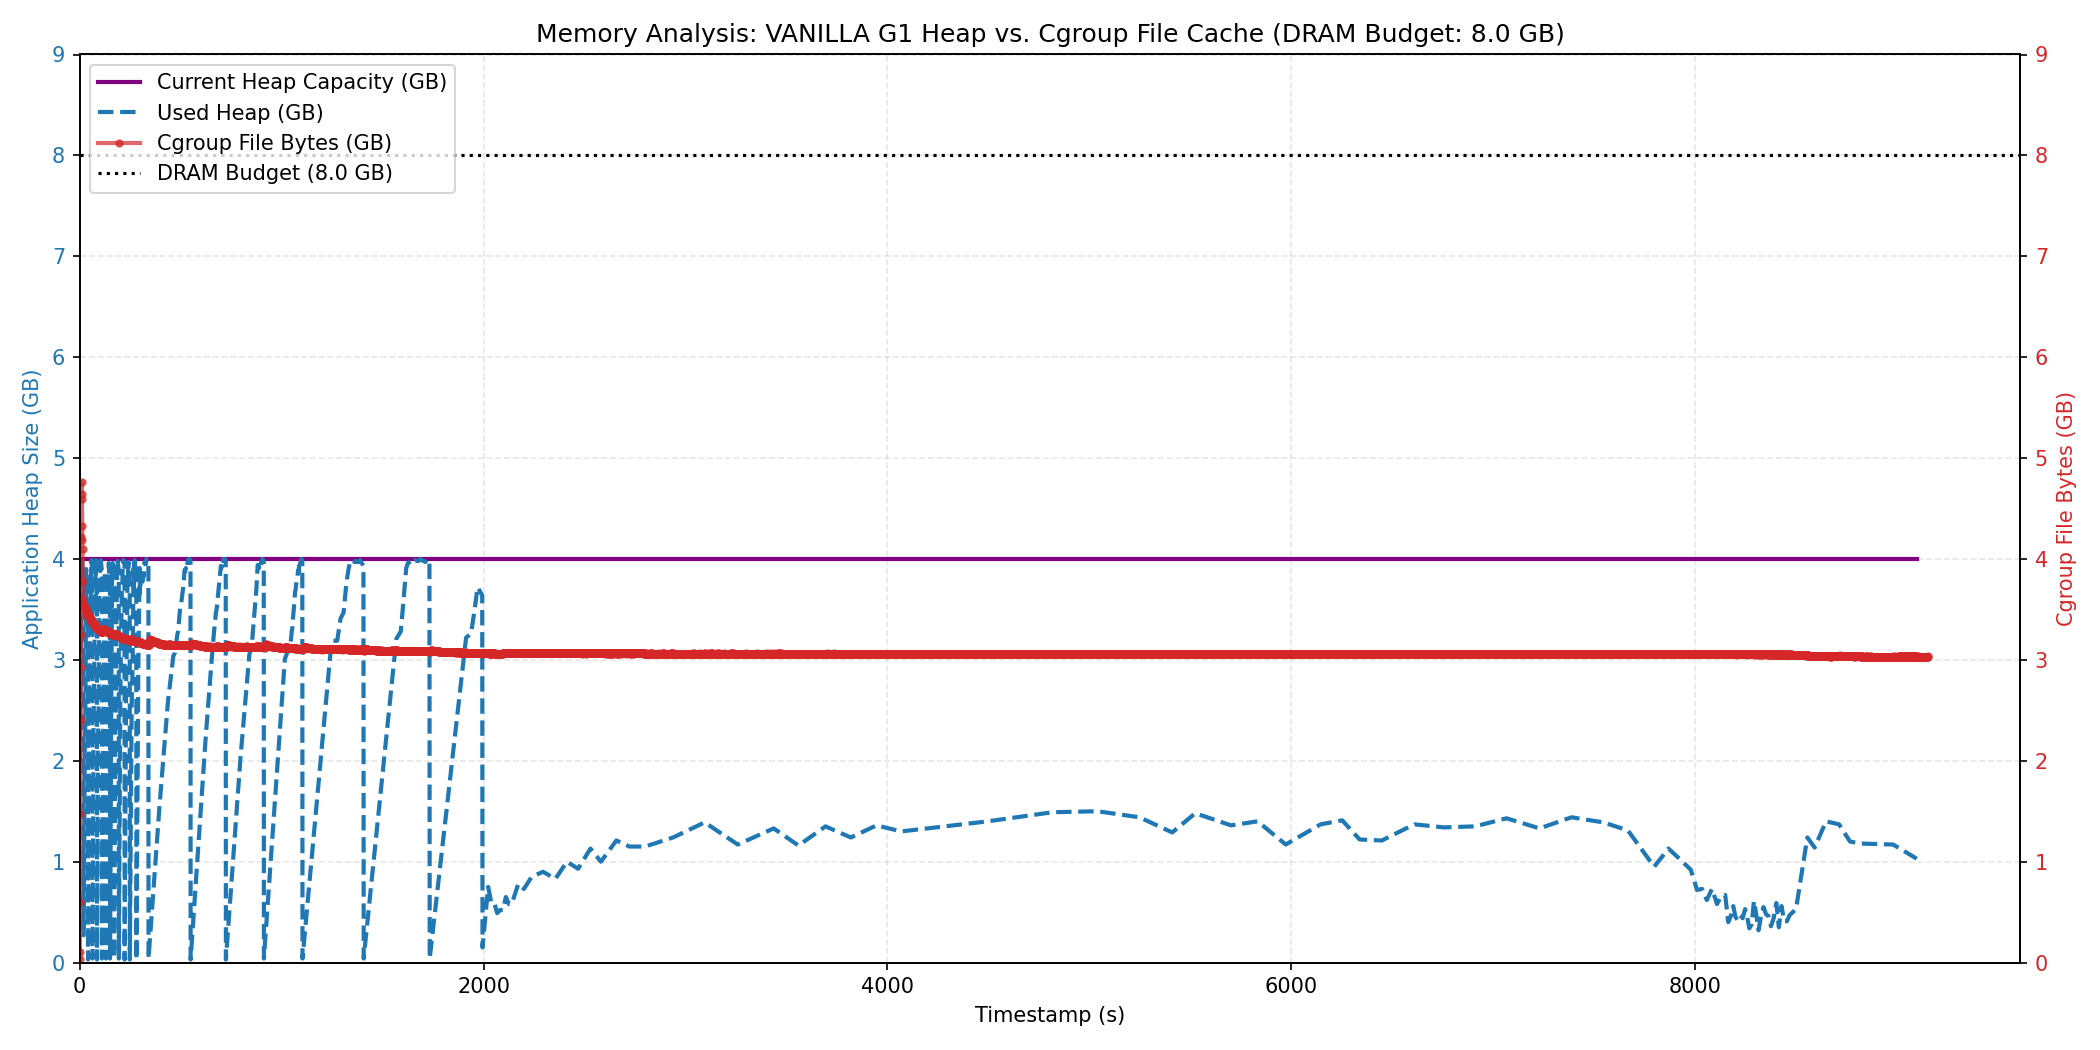
\includegraphics[width=\linewidth]{fig/combined_memory_timeline_vanilla_g1.png}
        \vspace{0.5em}
        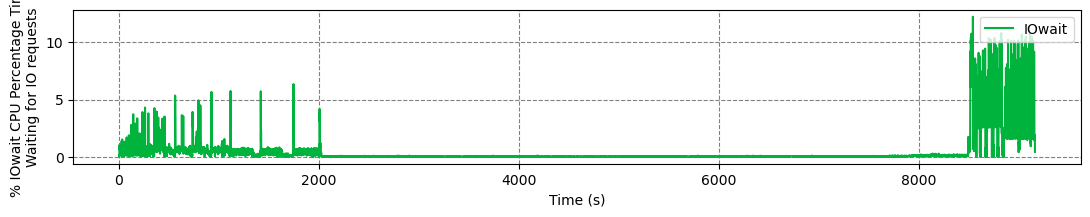
\includegraphics[width=\linewidth]{fig/iow_cpu_teraheap.png}
        \subcaption{M1 Lucene benchmark with 4\,G H1 and 4\,G page-cache}
        \label{fig:lucene-m1_th}
    \end{minipage}
    \hfill
    % Right column (Benchmark + IOWait)
    \begin{minipage}[t]{0.49\textwidth}
        \centering
        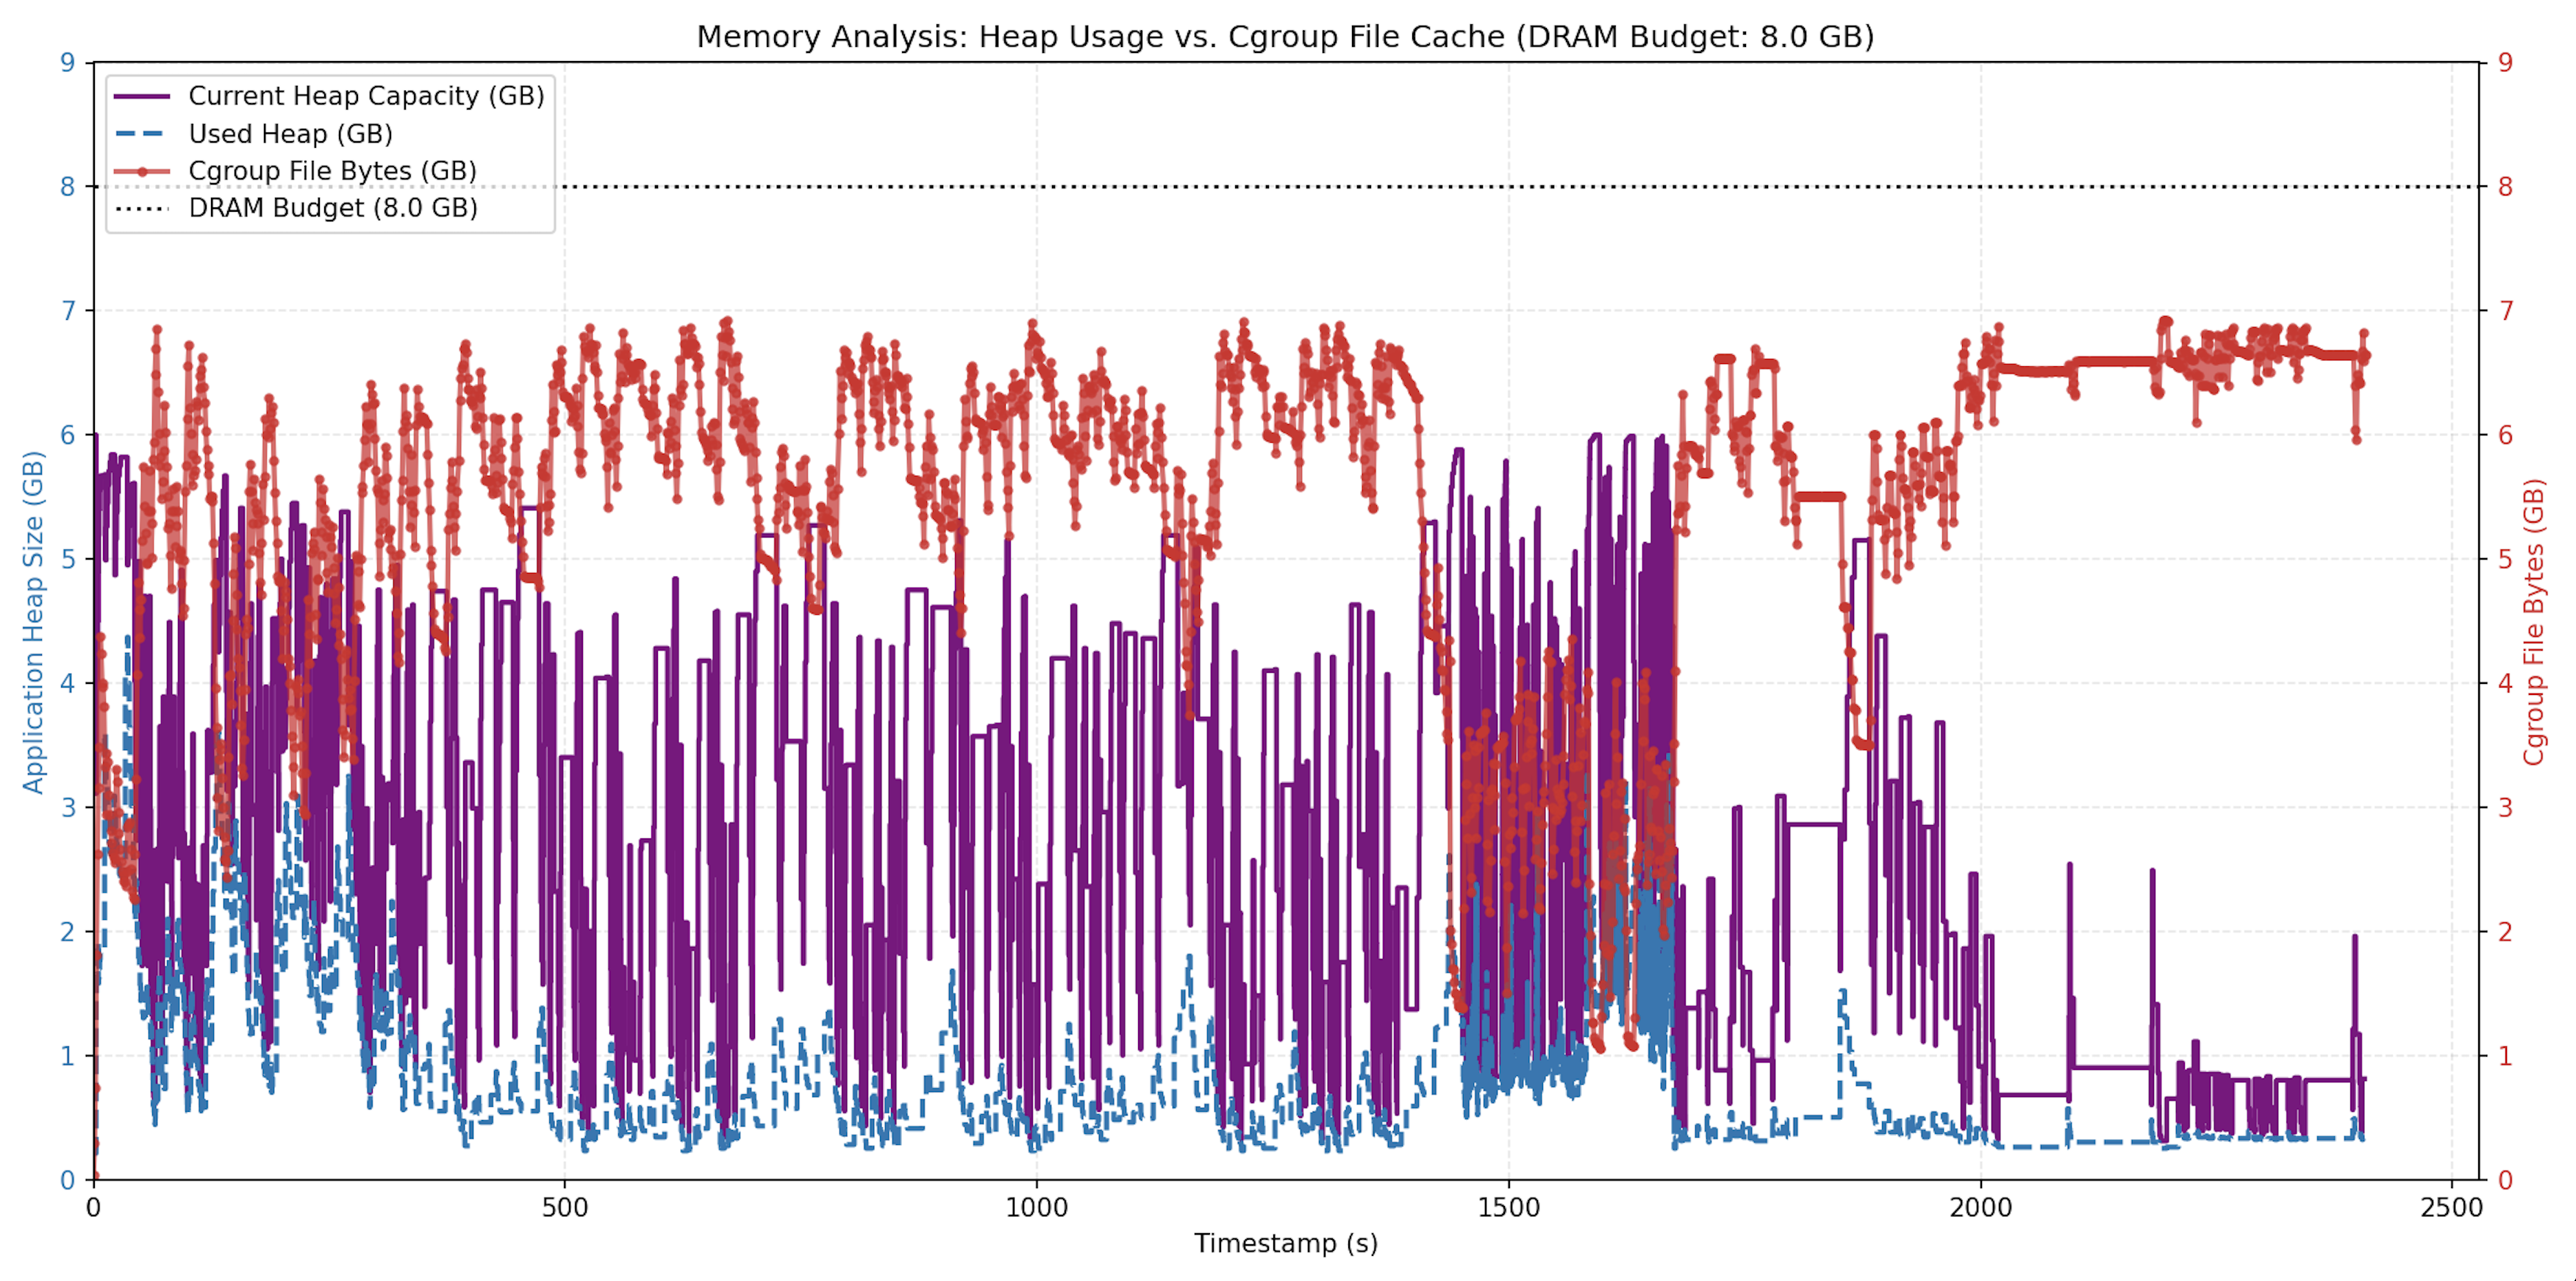
\includegraphics[width=\linewidth]{fig/flexheap_debug.png}
        \vspace{0.5em}
        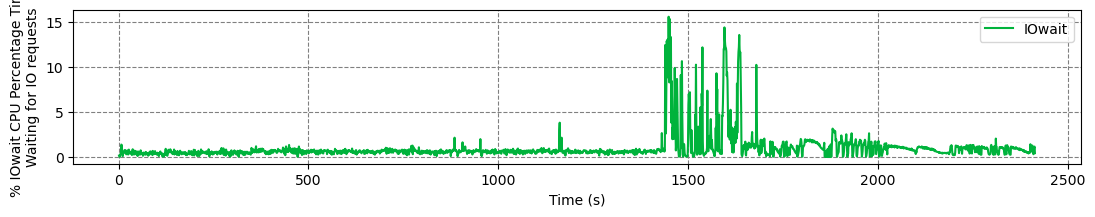
\includegraphics[width=\linewidth]{fig/iow_cpu_flex.png}
        \subcaption{M1 Lucene benchmark with 6\,G H1 and 2\,G page-cache}
        \label{fig:lucene-m1_flex}
    \end{minipage}

    \caption{Execution timeline (top) and I/O wait (bottom) for two M1 Lucene runs under static and dynamic DRAM partitioning.}
    \label{fig:lucene_m1}
\end{figure*}

To address this limitation, we port FlexHeap \cite{flexheap} to our system, a dynamic
resizing policy that operates at runtime by dividing execution into sampling
intervals. During each interval, it tracks the number of CPU time consumed by Garbage-Collection (GC)
and the I/O overheads including I/O caused by accesses to
the (H2) memory-mapped file. At the end of each interval, it compares the
percent change between the two metrics, relative to the previous intervals. If
garbage collection overhead has increased more than I/O stalls, FlexHeap
signals G1 to grow the H1 heap to relieve GC pressure. Inversely, if I/O delays
have increased, a shrink heap action is invoked, shifting the remaining memory
towards the pagecache, via cgroups, to reduce evictions and hold more data from
the H2 file.

Across Lucene and Spark benchmarks, FlexHeap achieves 
execution time improvements of up to 70\% and 9\%, compared to 
TeraHeap with static DRAM partitioning. We implement FlexHeap as an extension 
to OpenJDK 17, extending TeraHeap.
In this thesis we make the following contributions:

\vspace{0.5em}
\begin{itemize}
\item We identify and analyze the limitations of static DRAM partitioning in a tiered managed heap 
  environment, highlighting how fixed memory allocations can not optimize performance 
  due to underutilized memory and I/O pressure.

\item We intergate FlexHeap, into TeraHeap \cite{melidonis_thesis, mairh_thesis}.

\item We evaluate FlexHeap on real-world Lucene and Spark workloads, showing consistent
  performance improvements and better DRAM utilization under certain memory budgets.

\end{itemize}
